\chapter{Related Work}
\label{chapter:related.work}

The design of Warlock is based on well known distributed algorithms. We discuss
these algorithms here and list similar projects that meet few of our
requirements (\chapterref{requirements}).

\section{Paxos}
\label{section:paxos}

Paxos is regarded as the simplest and most obvious of distributed algorithms
\citep{Lamport01}. It is a consensus protocol used for replication of state
machines in an asynchronous environment \citep{Lamport98}. We use Paxos in this
thesis primarily since it has been shown that it has the minimal possible cost
of any consensus algorithm in the presence of faults \citep{KeidarR03}.

A consensus algorithm tries to get a group of processes to agree on a value
while satisfying its safety requirements%
\sidenote{
  Safety requirements of a consensus algorithm \citep{LamportM04}:
  \begin{inparaenum}[(i)]
    \item \emph{Non triviality}: A value has to be proposed to be chosen.
    \item \emph{Consistency}: Different learners cannot learn different values.
    \item \emph{Conservatism}: Only chosen values can be learned and it can be
      learned at most once.
  \end{inparaenum}
}.
These processes in the Paxos algorithm can be classified based on their roles
without affecting its correctness:

\begin{itemize}
  \iterm{Proposer}: A process that can propose values to the group.
  \iterm{Acceptor}: Acceptors form the \val{memory} of the algorithm that allows
  the algorithm to converge to a single value.
  \iterm{Learner}: The chosen values are \val{learned} by the other processes.
\end{itemize}

\begin{figure}
  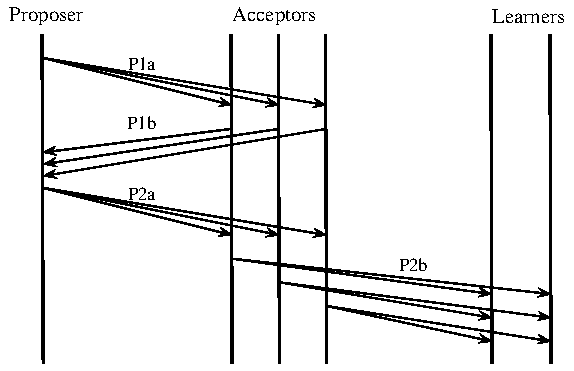
\includegraphics[width=0.6\wholewidth]{basic-paxos}
      \caption[Basic Paxos]{%
        Basic Paxos Algorithm: Processes with roles \dash{} Proposer, Acceptor,
        Learner \dash{} send messages to each other illustrating the flow of the
        algorithm in a failure free instance.}
      \label{figure:basic_paxos}
  \normalcaption
\end{figure}

The algorithm proceeds in two phases with each phase having two sub phases.

\begin{itemize}
  \iterm{Phase 1 a}: The proposer selects a number \code{n} and sends it as a
  \code{prepare} (\code{P1A}) message to all the acceptors.
  \iterm{Phase 1 b}: Each acceptor compares the \code{n} it
  receives and if it is greater than all previous numbers received as a part of
  \code{prepare}, it replies (\code{P1B}) with a promise not to accept any
  number lower than \code{n}.
  \iterm{Phase 2 a}: If the proposer receives a response to its \code{prepare}
  messages from a quorum%
  \sidenote{
    \emph{Quorum}: Majority agreement of processes. It is used to ensure
    liveliness in the system.
  }, it sends a reply (\code{P2A}) back to each of the acceptors with an
  \code{accept} message. The message also consists of the value \code{v}
  which is the highest numbered proposal among all the responses from the
  acceptors. In case it is empty, the proposer is free to choose the value.
  \iterm{Phase 2 b}: If the acceptor has not received \code{prepare} request
  with a larger number when it receives an \code{accept} request from the
  proposer, it sends a message (\code{P2B}) to the learner with the accepted
  value \code{v}.
  \iterm{Learner}: If the learner receives a message from a quorum of
  acceptors, it concludes that the value \code{v} was chosen.
\end{itemize}

The algorithm makes progress when a proposed value is eventually learned by all
the learners. However, a scenario where no progress can be made is possible
when we have multiple proposers.

Consider two proposers issuing \emph{prepare}
requests with alternatively increasing \emph{n}. They would keep
preempting each other in a loop leading to no agreement being reached among the
group. A solution is to create the role of \emph{distinguished proposer} or
\emph{leader} where it becomes the only process that can issue new requests.
\citet{FisLynPat85} implies the \val{election} of this \emph{leader}
should use either randomness or timeouts.

Although the pseudo-code of the algorithm is relatively small, implementing it
to create a stable, production ready system is non-trivial \citep{ChandraGR07}.
Different flavors of Paxos allows us to choose specific based on the project's
requirements.

The family of Paxos algorithms differ from each other based on the topology
of the process group, number of phases involved for one instance%
\sidenote[-2]{
  \emph{Paxos Instance}: Single run of the algorithm starting from the value
  being proposed to the learning of the value by the learners.
}, amount of message delays and so on. We explore some of these Paxos variants.

\subsection{Basic Paxos}

Basic Paxos is the simplest version of Paxos and is the same as described
previously in \sectionref{paxos}. The algorithm proceeds over several rounds
with the best case taking two rounds. It is typically not implemented and used
in production due to possible race conditions and relatively poor performance.

\subsection{Multi-Paxos}

We run one instance of Paxos algorithm for agreeing on a single value and
multiple times for multiple values. We can batch together multiple values
into a single instance, but this optimization does not reduce the message
complexity.

\emph{Phase 1} of the algorithm become
an unnecessary overhead if the \emph{distinguished proposer} remains the same
throughout. Multi-Paxos uses this as its basis to reduce the message count.
The first round of Multi-Paxos \citep{dumulti} is the same as Basic Paxos.
For subsequent values, the same
proposer starts directly with \emph{Phase 2} halving the message complexity.
Another proposer may take over at any point of time by starting with
\emph{Phase 1 a} overriding the current proposer. This is not a problem since
the original proposer can start again with \emph{Phase 1 a}.

\citet{Robbert2011} provides the imperative pseudo-code for Multi-Paxos and
the details required for making it practical. We use it as a
basis for implementing Paxos.

\subsection{Fast Paxos}

Fast Paxos \citep{MSRTR2005112} is a variation of Basic Paxos, It has two
message delays compared to four message delays of Basic Paxos and guarantees
the round to be over in three message delays in case of a collision.

Clients propose the values directly to the \emph{acceptors} and the
\emph{leader} gets involved only in case of a collision. Versions of Fast
Paxos can be optimized further by specifying the collision
resolution technique allowing the clients to fix collisions themselves.

However, according to \citet{Vieira08theperformance} and \citet{Junqueira2007},
Fast Paxos is not better than Basic Paxos in all scenarios. Basic Paxos was
found to be faster in case of systems with small number of replicas owing to
the stability provided by its use of a single coordinator and the variation
of message latencies in practical networks. Fast Paxos also needs larger quorum
sizes of active replicas for it to function.

\subsection{Cheap Paxos}

Basic Paxos requires a total of \code{2N+1} servers in a distributed system to
tolerate \code{N} failures. However, \code{N+1} servers are enough (minimum) to
make progress.
Using servers that are slower or cheaper for the additional \code{N} servers
allows us to reduce the total cost of the system. Cheap Paxos \citep{LamportM04}
is designed along these lines.

Cheap Paxos uses \code{N} auxiliary servers along with \code{N+1} main servers
which allows it to tolerate \code{N} failures. The idea is that the auxiliary
server steps in to replace one of the main servers when it goes down
temporarily. The main server takes back control once restored. The auxiliary
servers thus act as a backup to the main servers without actively taking part
in the protocol, merely acting as observers.

The downside of using Cheap Paxos is that it affects the liveliness of the
system when multiple main servers fail at the same time since it takes time
for the axillary servers to be configured into the system.

\subsection{Ring Paxos}

Ring Paxos \citep{MarandiPSP10} is based on the observations that messaging
using ip-multicast%
\sidenote{
  \emph{Ip-Multicast}: is the process sending messages to a group of receivers
  in a single transmission.
}
is more scalable and provides better throughput compared
to unicast%
\sidenote[2]{
  \emph{Unicast}: transmission of message to a single destination.
}
for a distributed system in a well-defined network. It
has the property that it provides fixed throughput with variation in number
of receivers. It claims to have the throughput of ip-multicast and low latency
of unicast with the downside being that it provides weak synchrony%
\sidenote{
  \emph{Weak synchrony}: Message loss is possible.
}.

\begin{figure}
  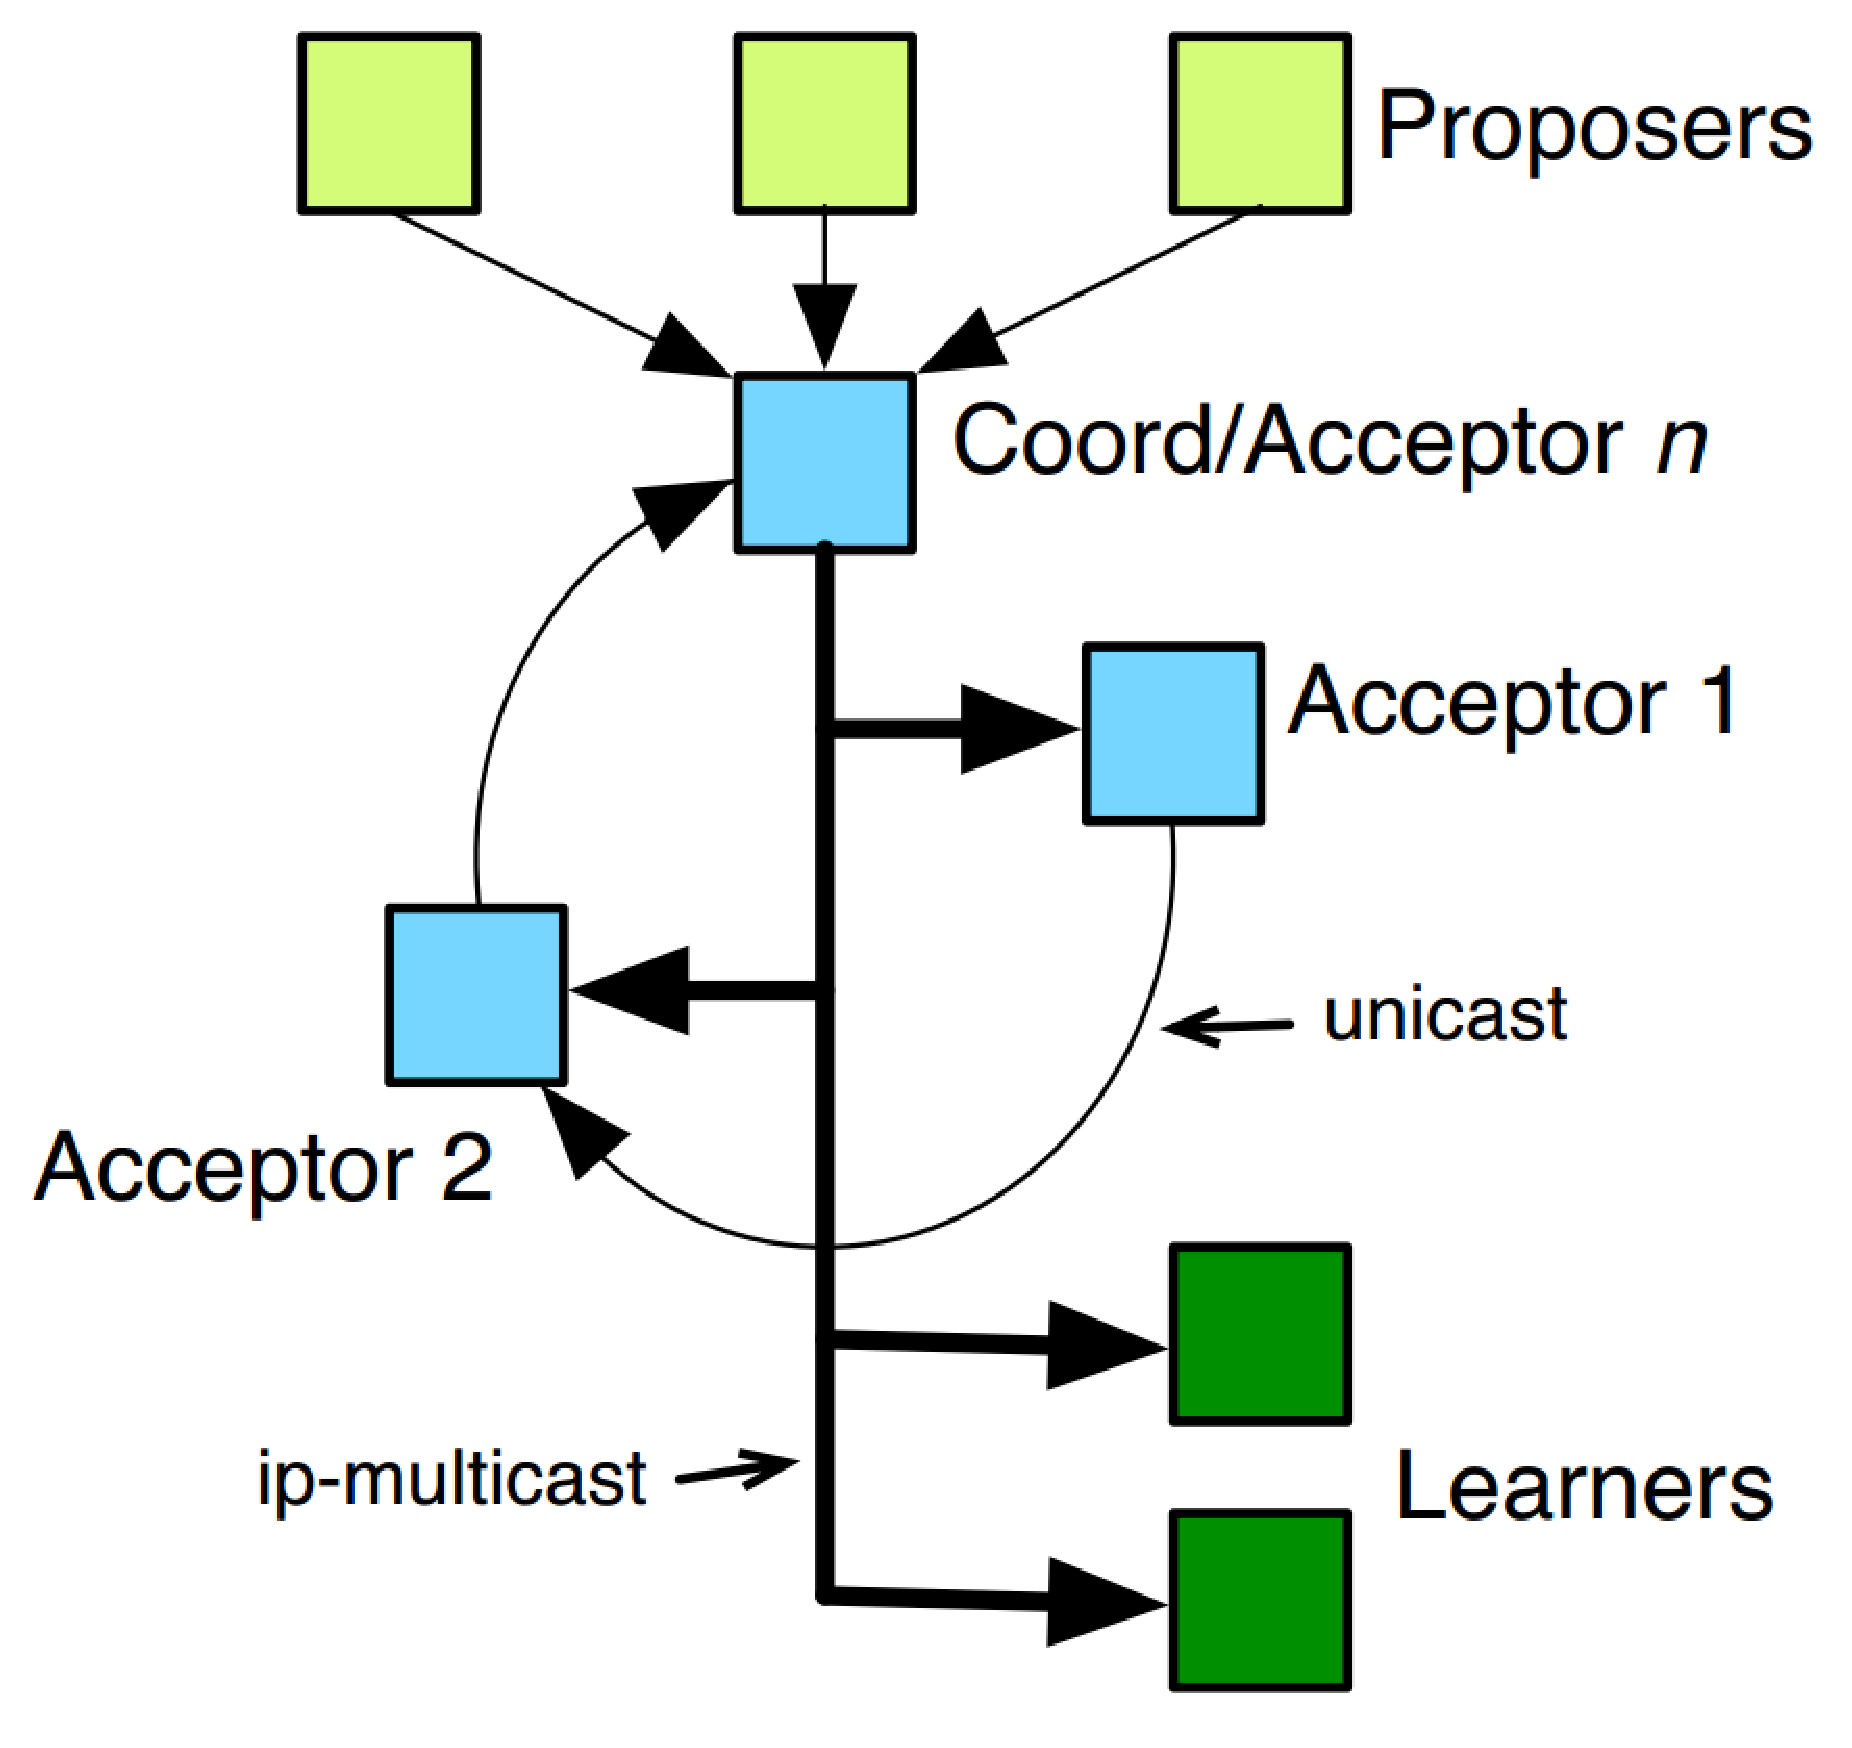
\includegraphics[width=0.5\wholewidth]{ring_paxos}
  \caption[Ring Paxos]{%
  Processes and their roles in Ring Paxos. Figure courtesy
  \citep{MarandiPSP10}.}
  \label{figure:ring.paxos}
\end{figure}

\figureref{ring.paxos} illustrates the outline of Ring Paxos algorithm and
shows the two communication protocols used between its processes.

\subsection{Stoppable Paxos}

The Basic Paxos algorithm is run under the assumption that all the participating
processes are fixed and form a static system. However, the system should
support cluster reconfiguration to be able to run for long periods of time in a
practical environment. Reconfiguration includes adding new servers,
removing/replacing old/faulty servers, scaling down the number of servers
when lower throughput is acceptable and so on.

Stoppable Paxos (\citet{LamportSP08}, \citet{LamportMZ10}) is one such algorithm
that allows us to reconfigure a Paxos based system. The algorithm defines a
special set of \emph{stopping} commands. A stopping command is issued as the
\code{i}th command after which no new command at \code{i+1}the position can be
issued. The system proceeds normally after it executes the \code{i}th command.

This thesis uses a variation of Stoppable Paxos for reconfiguration.

\subsection{Other}

Even though most of the Paxos papers detail the algorithm in pseudo code, it is
non trivial to actually implement it. A few papers detail the fine points to
consider from the implementation perspective.

\subsubsection{Paxos for System Builders}

\citet{Kirsch08paxosfor} provides a detailed overview of Paxos from the
implementation perspective. They list the necessary pseudo code required
along with all the considerations needed to make the algorithm practical.
Furthermore, they explore performance, safety and liveliness
properties of the prototype they built.

\subsubsection{Paxos Made Live \dash{} An Engineering Perspective}

\cite{ChandraGR07}
details the learning in engineering the Paxos algorithm for use in
Google Chubby Locks \citep{Burrows06}.

The paper details the experience of engineers from Google in building a
large scale system centered around Paxos. It details the major challenges faced
and their solutions, performance considerations, Software Engineering techniques
used and information of testing the setup.

\subsection{Implementations}

There are several implementations of Paxos and its variants. Listed below are
implementations written mainly in Erlang. These projects serve as a good
reference from the implementation perspective.

\subsubsection{gen\_paxos}

\citep{Uenishi2012} implements Paxos with
individual processes modelled as finite state machines. Each process can
be performing a different role based on what state it is on. This
makes all processes equal and ready to take on different roles
as required during runtime.

\begin{figure}
  \begin{whole}
  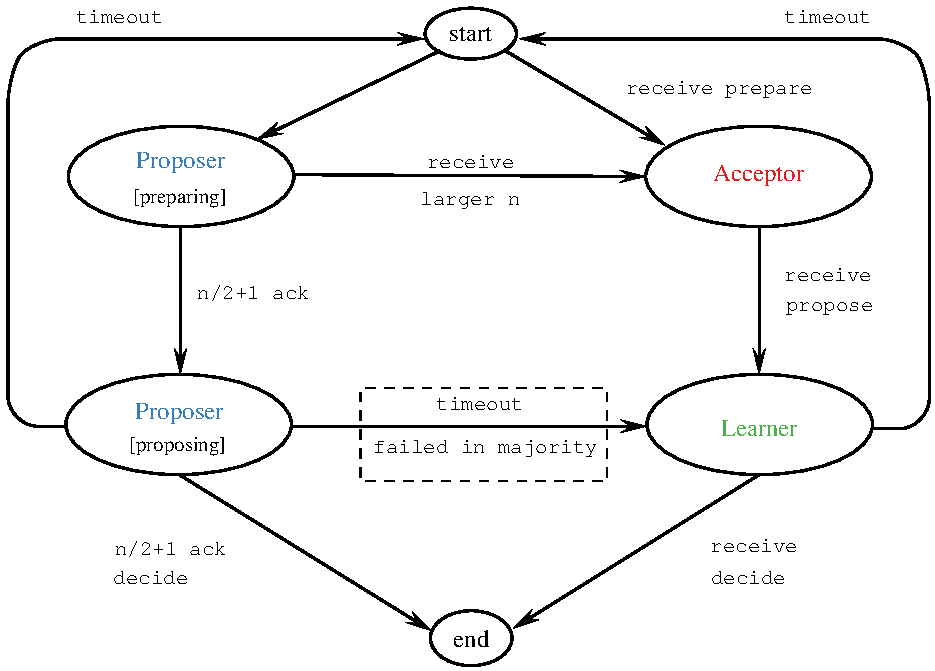
\includegraphics[width=1\wholewidth]{paxos_fsm}
  \caption[Paxos \abbr{FSM}]{%
    Figure shows Paxos algorithm when viewed as a finite state machine.}
  \label{figure:paxos.fsm}
  \end{whole}
\end{figure}

\figureref{paxos.fsm} shows the view of Paxos algorithm as a Finite State
Machine (\abbr{FSM}). The idea is that each process is run as an instance of
this \abbr{FSM}, contrary to the regular view of process with a single well
defined role. While this view of Paxos as a \abbr{FSM} is very helpful in the
understanding of the protocol, we chose to use the protocol in the already
established form of a single role per process.

\subsubsection{LibPaxos}

\citet{Lugano2012} is a collection of open source
implementations of Paxos created specifically for performance measurements
in \citet{MarandiPSP10}. It also includes a simulator written in Erlang to
observe network behaviour.

\subsubsection{gen\_leader}

\citet{Ulf2012} implements a leader election based on First In
First Out (\abbr{FIFO}) basis. It is one of the notable implementations for
leader election in Erlang.

\section{Google Chubby Locks}
\label{section:chubby.locks}

Google created Chubby lock service \citep{Burrows06} for loosely-coupled
distributed systems. It works as a distributed file system with advisory
locks%
\sidenote{
  \emph{Advisory Locks}: Long term locks used specifically within an
  application.
}. The goal of the project is to allow the clients to use the service
to synchronize their activities. For example, Google File System \citep{gfs}
and BigTable \citep{ChangDGHWBCFG06} use Chubby locks for co-ordination and
as a store for small metadata \citep{ChandraGR07}.

\begin{figure}
  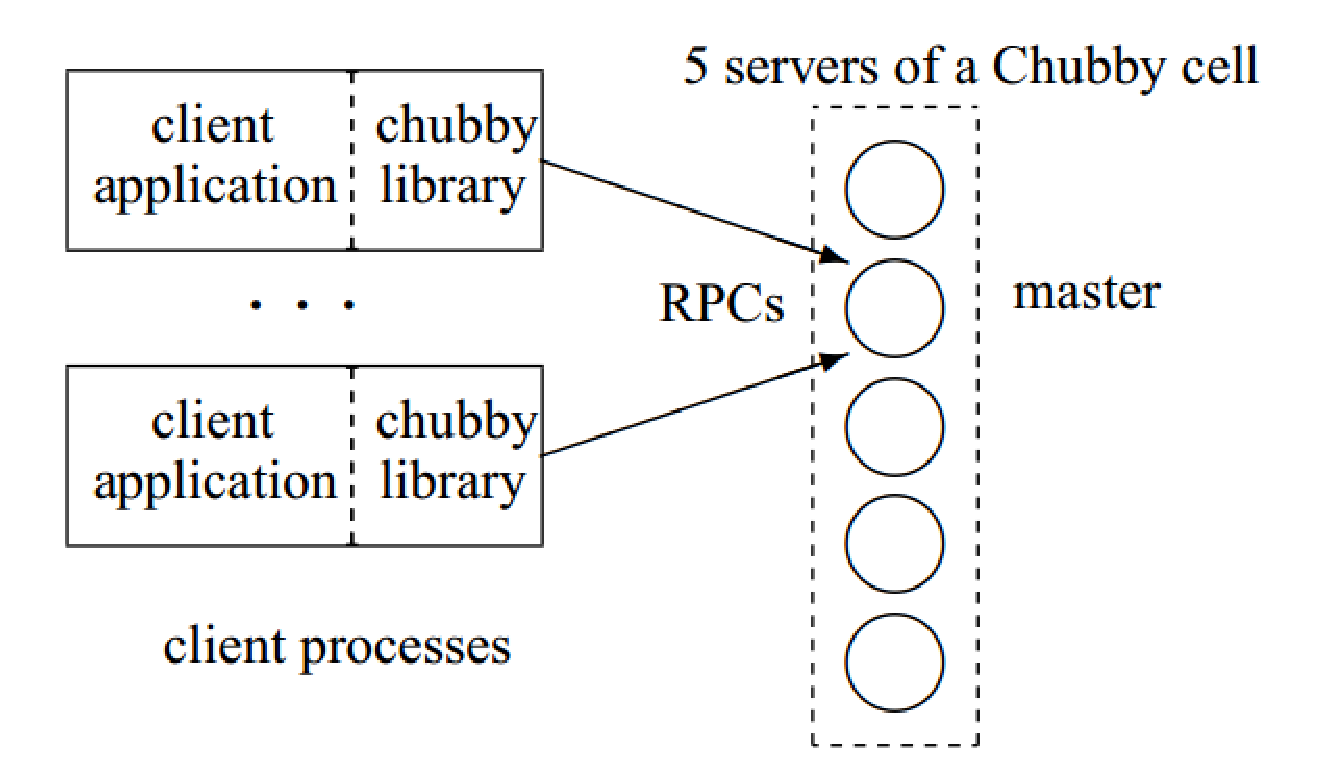
\includegraphics[width=0.5\wholewidth]{chubby_structure}
  \caption[Chubby structure]{%
    Figure shows the connection between Chubby cell and Chubby clients.
    Figure courtesy \citet{Burrows06}.}
  \label{figure:chubby.structure}
\end{figure}

Chubby lock is made up of two components:

\begin{itemize}
    \iterm{Chubby Cell}: Chubby cell is typically made up of five servers
    (termed replicas) that elect a master using Paxos protocol. The master
    server serves all the reads requests and co-ordinates the writes requests.
    The rest of the servers are for fault tolerance and are ready to replace the
    master should it fail.
    \iterm{Chubby Client}: Chubby client maintains an open connection with
    the Chubby cell and communicates with it via \abbr{RPC}%
    \sidenote{
      \emph{RPC}: Remote Procedure Call: An inter-process communication
      technique where one process can run programs on remote processes.
    }
    . The client maintains an in-memory write though cache that
    is kept consistent by the master using invalidations. The client is
    aware of the cell status using special requests%
    \sidenote[1]{
      \emph{KeepAlives}: Periodic requests used for indicating status.
    }
    .
\end{itemize}

\figureref{chubby.structure} shows the network connection between Chubby cell
 and Chubby clients.

\begin{figure}
  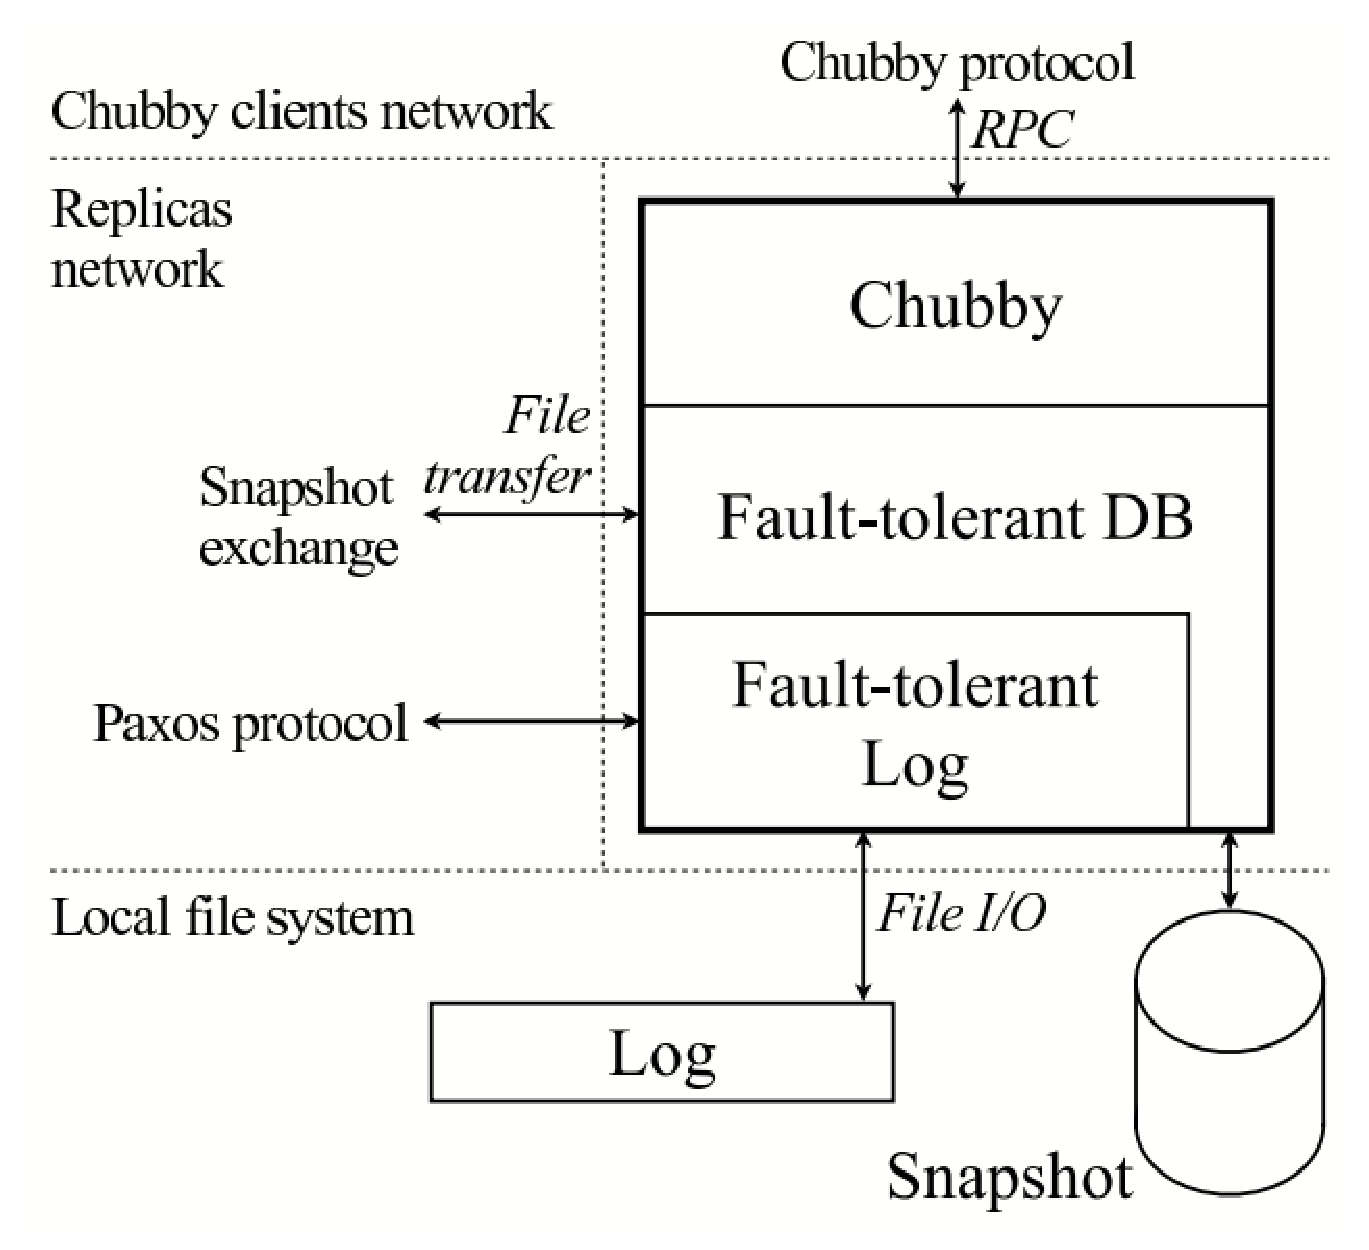
\includegraphics[width=0.5\wholewidth]{chubby_replica}
  \caption[Chubby Replica]{%
    Figure shows the internal of a single replica inside the Chubby cell.
    Figure courtesy \citet{ChandraGR07}.}
  \label{figure:chubby.replica}
\end{figure}

A Chubby replica, shown in \figureref{chubby.replica}, mainly consists of a
fault tolerant log that is consistent
with other replicas in the cell by using Paxos protocol. The rest of the
replica is made of a fault tolerant database and an interface to handle
requests from Chubby clients. The specific Paxos flavor used is Multi-Paxos
with slight modifications such as having a \val{catch-up} mechanism for
slower replicas.

The presence of the Chubby locks project and its use in some of the largest
server installations is a testimony of the need for distributed lock
managers. This thesis uses some of the ideas explored in Chubby locks, such
as using the Paxos protocol to agree on a callback function that can
eventually be run on the database component.

\section{Google Megastore}

Megastore \citep{BakerBCFKLLLLY11} is an \abbr{ACID}%
\sidenote{
  \abbr{ACID} properties are used to provide guarantees for database
  transactions.
  \begin{inparaenum}[(i)]
    \iterm{Atomicity}: A transaction is either executed completely or not
    executed at all.
    \iterm{Consistency}: The state of the database remains consistent after
    the transaction has been completed.
    \iterm{Isolation}: Transactions executed in parallel results in the same
    state as running all the transactions serially.
    \iterm{Durability}: All changes made by a transaction to a database is
    permanent.
  \end{inparaenum}
}
compliant, scalable datastore that guarantees high availability and
consistency. It uses synchronous replication for high availability and
consistent views while targeting performance by partitioning the data.

\begin{figure}
  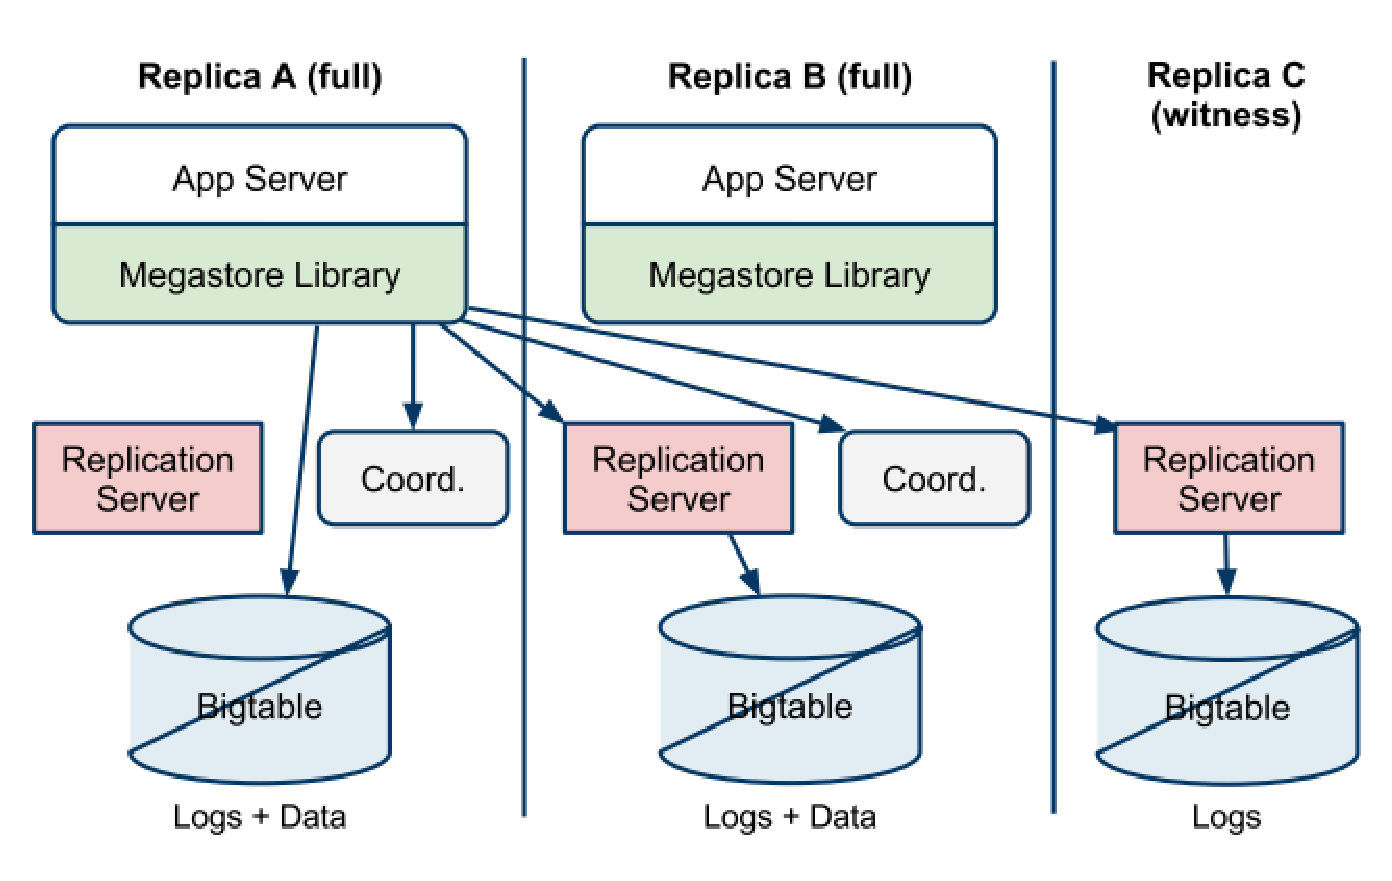
\includegraphics[width=0.6\wholewidth]{megastore}
  \caption[Google Megastore]{%
    Figure shows the example architecture for Google Megastore.
    Figure courtesy \citet{BakerBCFKLLLLY11}.}
  \label{figure:megastore}
\end{figure}

Megastore users Paxos to replicate a write-ahead log, replicate commit
records for single phase \abbr{ACID} transactions and as a part of fast fail
over
mechanisms. It provides fast local reads using a service called the
\emph{coordinator} which keeps track of the data version/Paxos write
sequence over the group of replicas. It speeds up writes by pre-preparing
optimizations and other heuristics.

\figureref{megastore} shows the core architecture of Megastore. It illustrates
the relation between different replicas and the coordinator.

\section{Apache Zookeeper}
\label{section:zookeeper}

Zookeeper \citep{Hunt:2010:ZWC:1855840.1855851, zookeeper} is a open source
consensus service written in Java that is used for synchronization in
distributed applications and as a metadata store. It is inspired by Chubby lock
\sectionref{chubby.locks}, but uses its own protocol Zookeeper Atomic Broadcast
(\abbr{ZAB}) in place of Paxos.

\subsection{Zookeeper Atomic Broadcast}

Zookeeper Atomic Broadcast (\abbr{ZAB})
\citep{Reed:2008:STO:1529974.1529978, JunqueiraRS11} is a
totally ordered atomic broadcast protocol created for usage in Zookeeper.
\abbr{ZAB} satisfies the constraints imposed by Zookeeper viz.,

\begin{itemize}
    \iterm{Reliable delivery}: Message delivered to one server must eventually
    get delivered to all the servers.
    \iterm{Total order}: Every server should see the same ordering of the
    delivered messages.
    \iterm{Causal order}: Messages should follow causal%
    \sidenote{
      \emph{Causal Ordering}: If message \emph{a} is delivered before message
      \emph{b} on a server then all other servers in the group should receive
      message \emph{a} before \emph{b}.
    }
    ordering.
\end{itemize}

\abbr{ZAB} is conceptually similar to Paxos, but uses certain optimizations and
trade-offs. The service using \abbr{ZAB} has two modes of operation:

\begin{itemize}
    \iterm{Broadcast mode}: Broadcast mode begins when a new leader is chosen
    using a quorum from the group. The leader's state is now same as rest of
    the servers and can hence start broadcasting messages.
    This mode is similar to two-phase commits \citep{Gray78}, but with quorum.
    \iterm{Recovery mode}: A new leader has to be chosen when the existing leader
    is no longer valid. The service is now in recovery mode until a new leader
    emerges using an alternative leader election algorithm.
\end{itemize}

\begin{figure}
  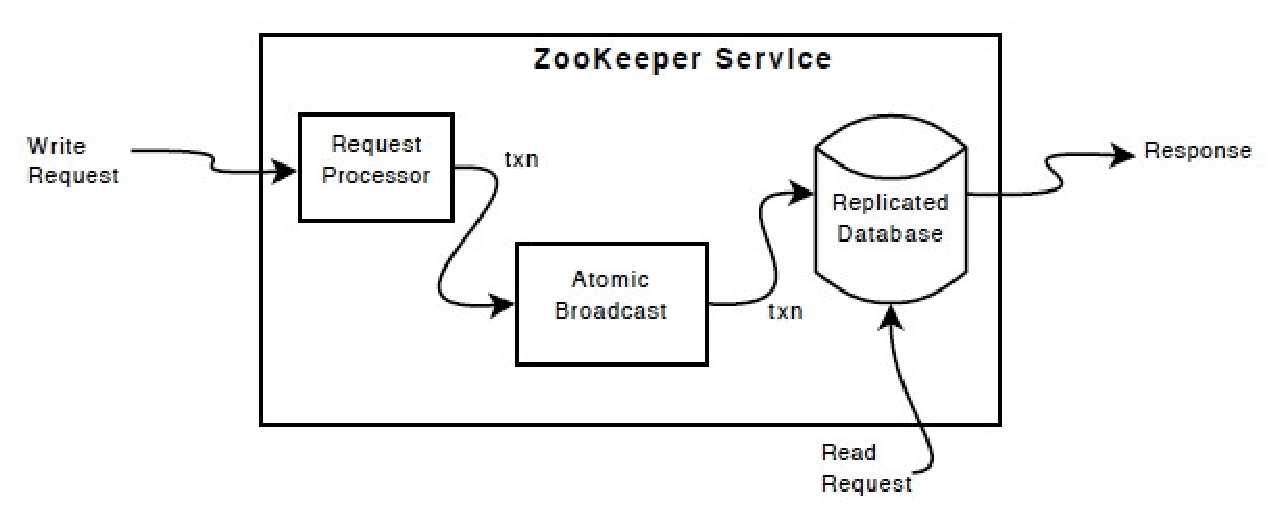
\includegraphics[width=0.7\wholewidth]{zkcomponents}
  \caption[Zookeeper Components]{%
    Figure shows the components of Zookeeper and the messaging between them.
    Figure courtesy \citet{zookeeper}.}
  \label{figure:zookeeper}
\end{figure}

\figureref{zookeeper} shows the message flow between different components inside
Zookeeper. We observe the optimization for \emph{read} requests, which allows it
to be much faster than the \emph{write} requests.

Zookeeper uses the concept of \emph{observers} to increase read throughput. They
are a set of servers that monitor the Zookeeper service, but do not take part
in the protocol directly thus acting as extended replicas. The write throughput
is however inversely proportional to the number of servers in the group mainly
due to the increased co-ordination required for consensus.

The data model of Zookeeper is that of a generic file system, which allows it
to be used as a file system as well. It provides features such as access
controls, atomic access, timestamps and so on.

Zookeeper worked on a static set of servers with no option to reconfigure the
cluster at the time of writing. However, the feature was in the works
\citep{zab2012} and an initial release was available.

\section{Doozerd}

Doozerd \citep{doozerd} is a consensus service similar to Chubby locks
\sectionref{chubby.locks} and Zookeeper \sectionref{zookeeper} written in
Go \citep{golang}. It uses Paxos protocol internally for maintaining
write consistency. Its use case is similar to that of Zookeeper and is
mainly used as a fast name service. However, it is not as widely used
or actively maintained as Zookeeper.

\section{Riak}

Riak \citep{riak} is a distributed eventually consistent datastore written in
Erlang. It is based on the concepts from Amazon's Dynamo \citep{DeCandia07}.

\begin{figure}
  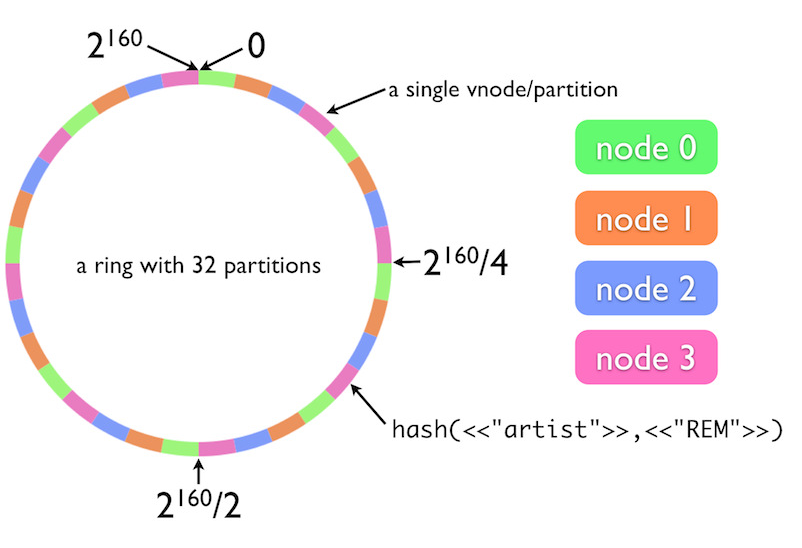
\includegraphics[width=0.7\wholewidth]{riak-ring}
  \caption[Riak Ring]{%
    Figure shows the Riak Ring and details how the key space is divided among
    four nodes
    Figure courtesy \citet{riak}.}
  \label{figure:riak.ring}
\end{figure}

The primary use of Riak is as a distributed NoSQL%
\sidenote[-4]{NoSQL, generally called \val{Not Only SQL} or
  \val{Not Relational}, are set of data stores that follow weaker
  consistency model than \abbr{ACID} and are characterized by their ability to
  scale their operations \citep{Cattell10}.
}availability and partition tolerance while
being eventually consistent. \figureref{riak.ring} shows the distribution of the
key space over multiple nodes using vnodes%
\sidenote{
  \emph{Vnodes} or \val{Virtual Nodes} are a level of indirection used to map
  the key space so that any change in the status of the physical node does not
  affect the key distribution.
}. It might be possible to use this concept to scale key space and avoid having
to store a complete copy of the data on all the nodes.

Riak is written in Erlang and is hence useful from this project's perspective
for providing a good conceptual view of building distributed database
applications in Erlang.

While the project is mature and satisfies all
the other requirements to be used as a lock manager, absence of strong
consistency makes its use untenable.

\section{Dynamo DB}

Amazon DynamoDB \citep{dynamoDB} is proprietary key-value datastore based on
\citet{DeCandia07} available as a service. While providing the regular
feature set of NoSQL data stores, it also provides strong consistency and
atomic counters. While DynamoDB satisfies most of this project's requirements,
usage of Warlock reduces the latency and provides quicker performance.

\section{Scalaris}

Scalaris \citep{scalaris} is distributed key-value database the supports
consistent writes and full \abbr{ACID} properties. It is based on Distributed
Hash Table (\abbr{DHT})%
\sidenote[-1]{
  \emph{Distributed Hash Table}: \abbr{DHT} is a distributed system that
  provides hash table operations.
}
and is implemented in Erlang. It also uses a non-blocking Paxos for consensus
and provides strong consistency. It uses a Peer to Peer (P2P) protocol \dash{}
Chord \citep{StoicaMKKB01} for its underlying data replication.

For our purpose however, Scalaris is a full featured database server with most
of the features being left unused. Because of this, it affects its performance
and needs more hardware for the necessary throughput.

